\chapter{User Study}

\section{Participants}
In total, 25 volunteers participated in this study, where 13 of them were male and 12 female students. The sample was drawn from university populations having an age range from 19 to 31 years with a mean age of M = 26.12 (SD = 3.1). Participants were selected from various discipline areas (see Figure~\ref{fig:Dfields}). We consider academic disciplines as three categories (Social, Natural and Formal Science) where almost 30\% of participants are from social sciences and 70\% from formal sciences. Moreover, the participants had a different education levels: the majority of them were studying Masters’s degrees, and only 32 percent were Bachelors’s and Ph.D. level students (see Figure~\ref{fig:DstudyLevels}).

\begin{figure}[H]
  \centering
    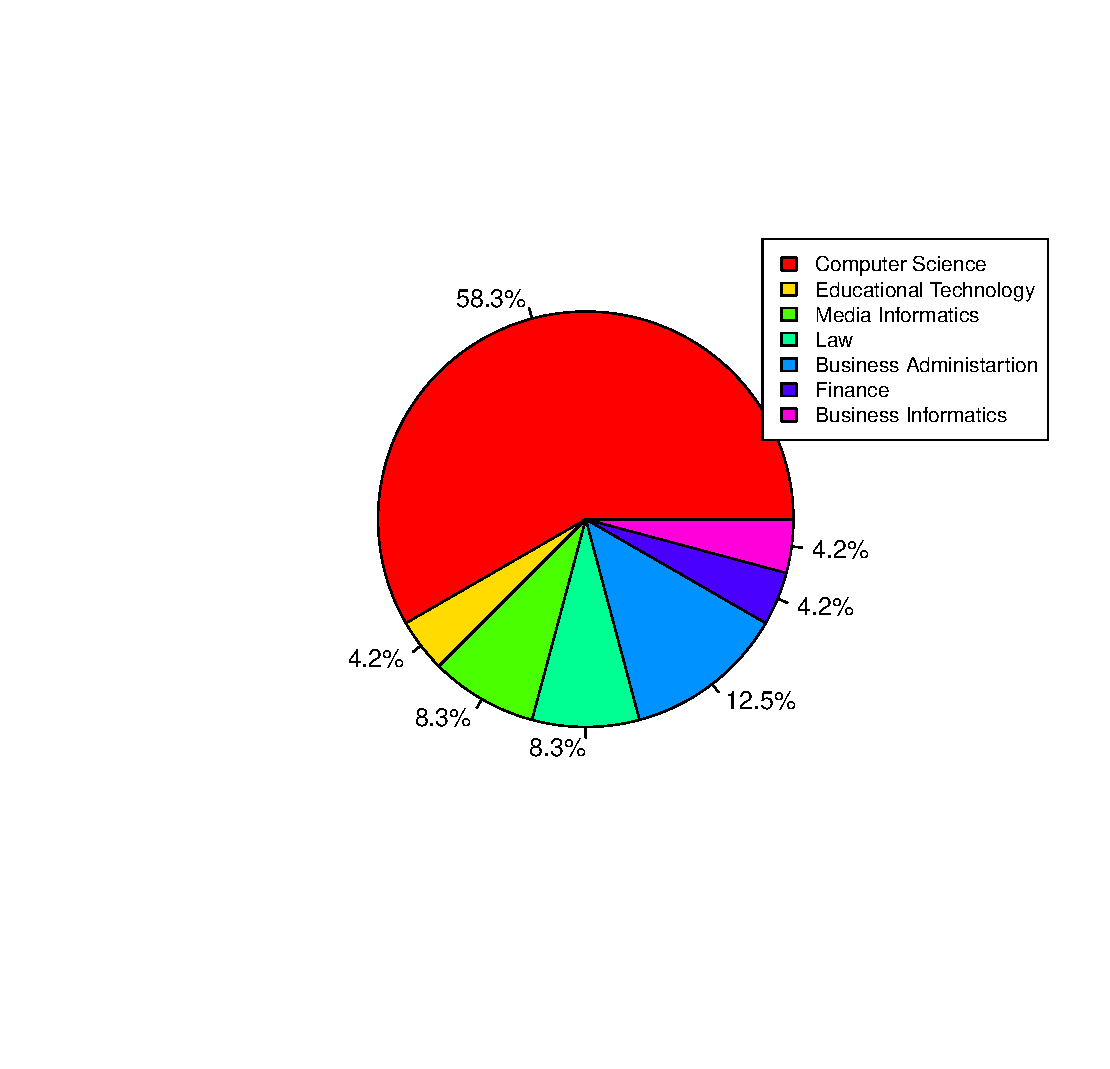
\includegraphics[scale=0.45]{RplotDemographicsFields.pdf}
      \caption{Participants' majors obtained from Demographics questionnaires}
      \label{fig:Dfields}
\end{figure}

\begin{figure}[H]
  \centering
    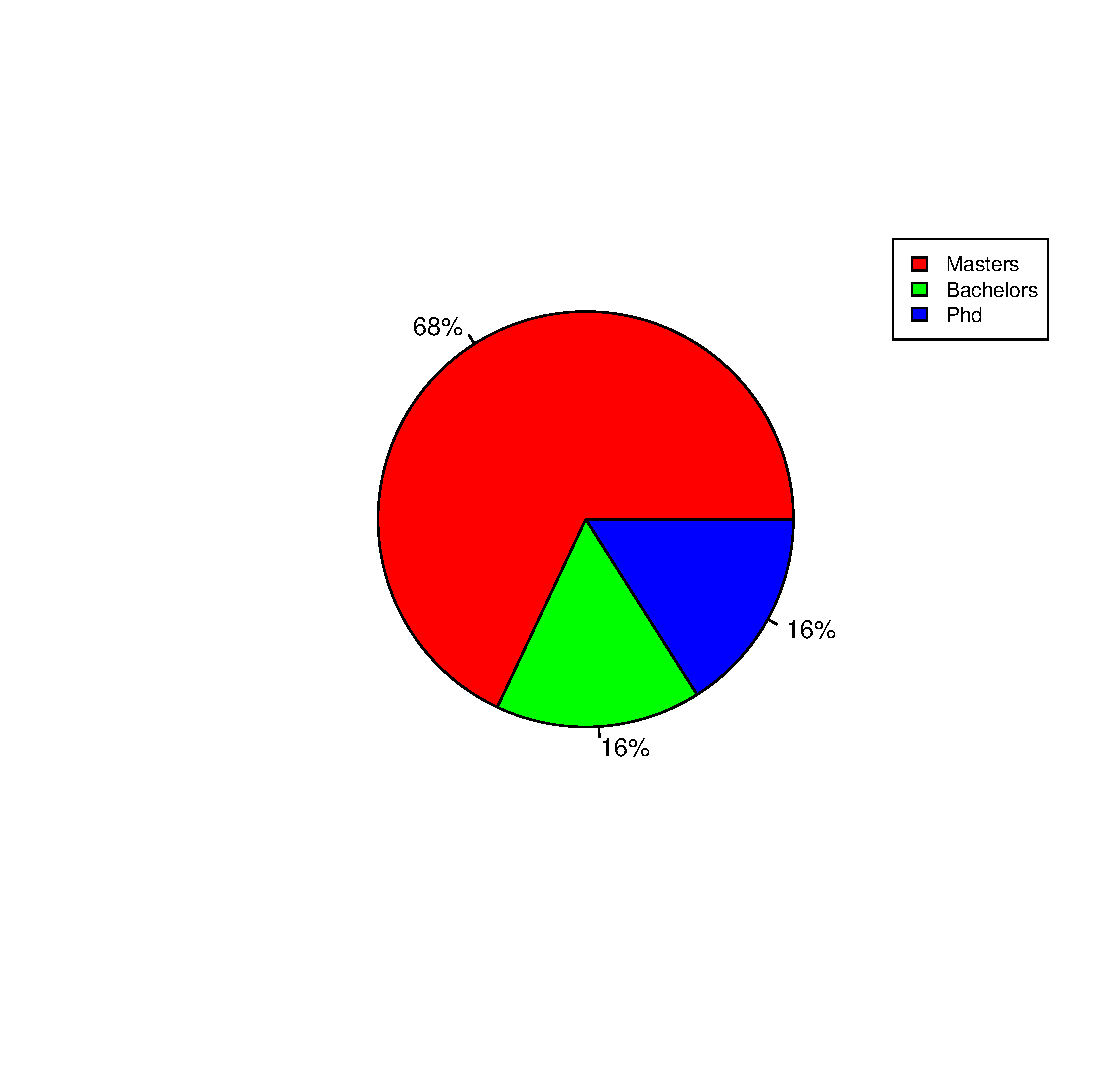
\includegraphics[scale=0.45]{RplotDemographicsStudyLevel.pdf}
      \caption{Participants' education level obtained from Demographics questionnaires}
      \label{fig:DstudyLevels}
\end{figure}

In the demographics form, participants also informed how frequently they used such devices as phones, smart lamps, tablets, and speakers (see Figure~\ref{fig:DdeviceUse} and Figure~\ref{fig:DdeviceUseInHours}). 

\begin{figure}[H]
  \centering
    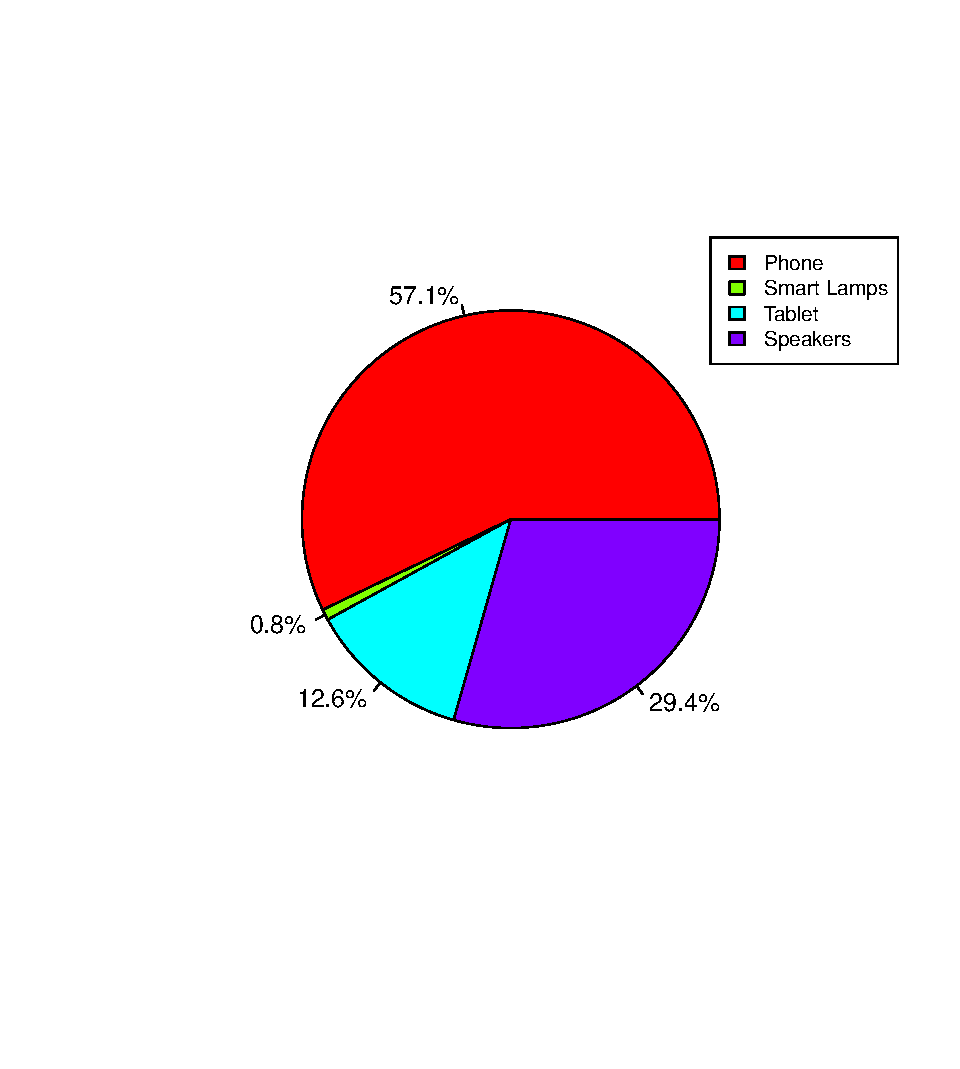
\includegraphics[scale=0.45]{RplotDemographicsDeviceUse.pdf}
      \caption{Participants' use of devices obtained from Demographics questionnaires}
      \label{fig:DdeviceUse}
\end{figure}

Overall, the experience level with above mentioned devices is listed in descending order: phone, speakers, tablet, and smart lamps. Figure~\ref{fig:DdeviceUseInHours} shows how many hours participants spend on these devices per day. The demographics questionnaire showed that the most popular device among our participants were phone with approximately 1/3 of participants who spent more than 6 hours on them. In all time ranges, the speakers were the second most used devices in comparison to the number of participants using of Tablet and Smart Lamps. 

\begin{figure}[H]
  \centering
    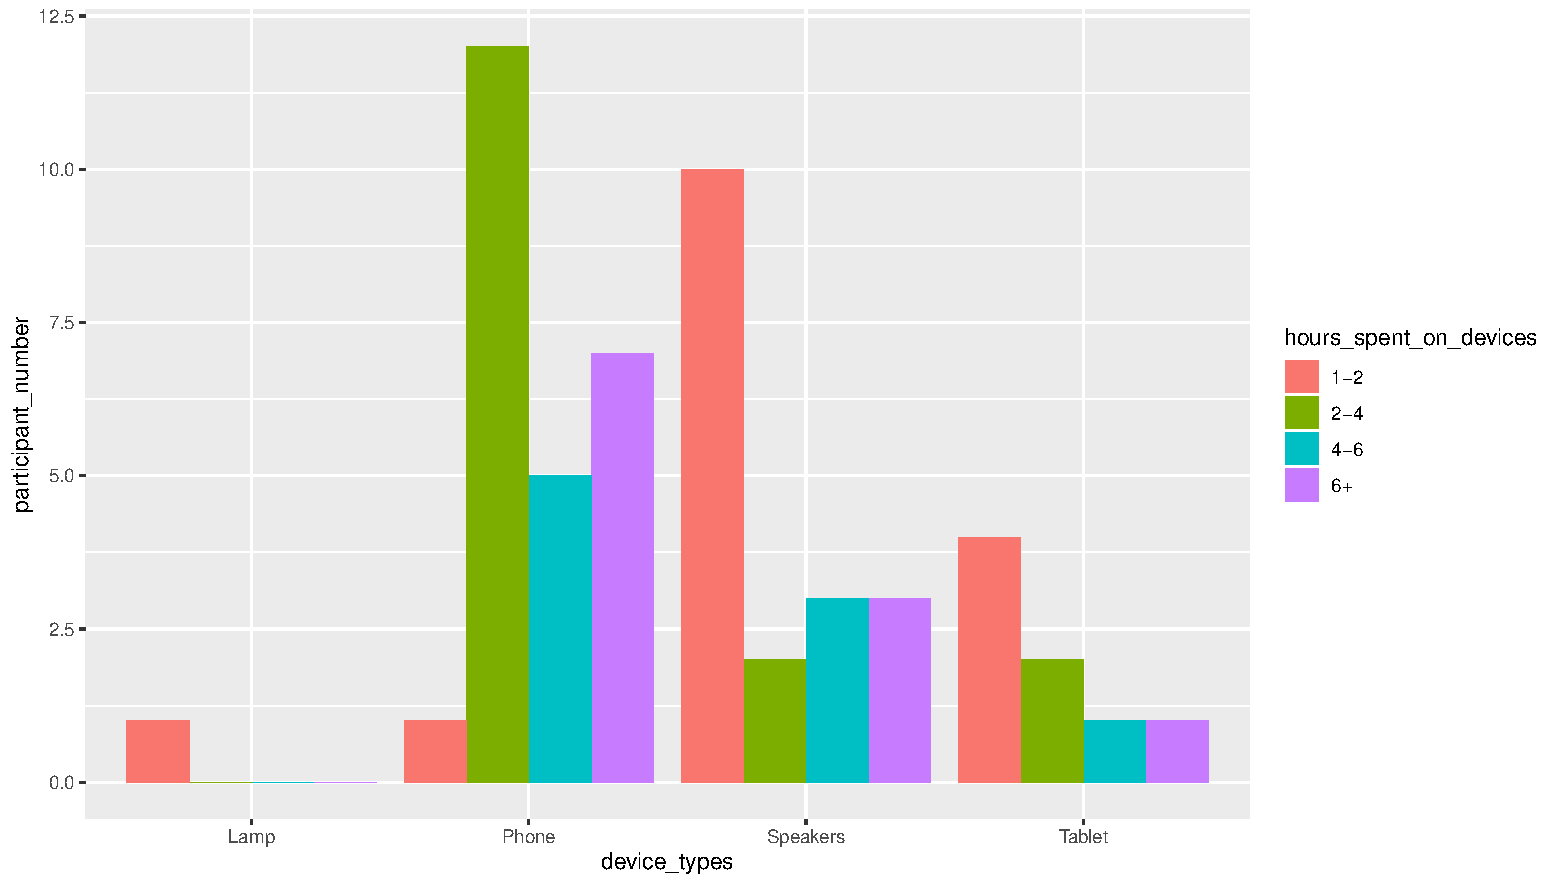
\includegraphics[scale=0.45]{RplotDemographicsDeviceUseInHours.pdf}
      \caption{Participants' device use in hours obtained from Demographics questionnaires}
      \label{fig:DdeviceUseInHours}
\end{figure}

In addition, Table~\ref{table:MusicFamiliarity} describes the participants’ preference of the music genres. The more fluent the participant would be with the music, the more rapid becomes the assessment of genre-specific features [Gjerdigen, R.O., Perrot, D., 2008. Scanning the dial: the rapid recognition of music genres]. Moreover, if the majority of participants prefer to listen or like certain genre of music, it may result in biased opinions. The mascot that triggers genre that they prefer may give participants more positive impression about their personality. Thus, the main reason of gathering data regarding participants' the music preferences was to see whether the liking factor affects the study or not. 
\par According to the One-Sample t-test with p>0.05, there was no significant effect of the participants’ music preference on the music genres that we chose for our study. Thus, we have insufficient evidence to conclude that one music genre is more preferable than the other. Meaning that, among the genres of music that we have chosen for our experiments, there were no distinguishably favorite genres and the participants had different music tastes (see Table~\ref{table:MusicFamiliarity}).

\begin{table}
\centering
\begin{tabular}{ | m{4.5em} | m{3em} | m{1em} | m{2em} | m{4em} | m{5.5em} | m{5em} |  } 
\hline
\multirow{2}{*}{} &
  \multicolumn{1}{| c}{ t-value} &\multicolumn{1}{| c}{df}  & \multicolumn{1}{| c}{mean} & \multicolumn{1}{| c}{p-value} & \multicolumn{2}{| c |}{95 percent confidence interval} \\
\hline
& 	&	&	  &  & lower & upper \\
\hline 
Country &	1 & 24 &	0.04 &	0.3273 &	- 0.04255594 & 0.12255594 \\
\hline 
Pop & 3.6742 &	 24 &	0.36	& 0.001195 &	0.1577801	& 0.5622199 \\
\hline 
Hip-hop	& 1.8091	& 24	& 0.12	& 0.08299	& - 0.01690354	& 0.25690354 \\
\hline 
Rap	&1&	24 &	0.04	& 0.3273 &	- 0.04255594&	0.12255594\\
\hline 
Jazz & 2.4495 & 24 &	0.2 & 	0.02198 & 	0.03148339 &	0.36851661\\
\hline 
Classic &	3.0551 &	24 &	0.28 &	0.005443 &	0.09084057	& 0.46915943\\
\hline 
Rock\&Roll	 & 1	& 24	& 0.04	& 0.3273	& - 0.04255594	& 0.12255594\\
\hline 

\end{tabular}
\caption{T-test for participants' familiarity with music genres used in our study}
\label{table:MusicFamiliarity}
\end{table}


\section{Procedure and Tasks}
When the experiment started, first, the participants were given an introductory paper describing the following aspects:
\begin{itemize}
  \item The implemented prototype introducing the devices used in our study
  \item The key idea of a study
  \item The purpose of the experiment
  \item The goal of the participants during experiment
  \item The number of phases and the overall duration of the experiment
\end{itemize}

Regardless of the introductory paper, the participant was allowed to ask open questions. After agreeing and signing the consent form (see appendix A), the main part of the experiment took place. 
\par In general, we have 4 phases for each of interaction types: Mascot-Mascot, Mascot-Lamps, Mascot-Tablet, Mascot-Speakers. The order of all phases were counterbalanced by using Latin Square. Each phase consists of 5 videos with a duration of 20 seconds, with the exception of Mascot-Speakers interactions where we have 9 videos with duration 40 seconds long. Moreover, for each participant, there were a different order of displaying the videos which are also randomized inside each phase based on the Latin Square. All phases and all videos within those phases were counterbalanced across all participants. Moreover, each participant was tested alone to ensure that the opinions of other participants do not affect their own. 
\par Before each phase, we describe the participant what kind of interaction they should expect from video and remind them their goals during that experiment. The goal is that, after watching short videos, participants will need to evaluate the personality of a Mascot according to the interaction that they have seen in the videos. When accomplishing watching the video, the participants were given a questionnaire (see appendix B) with 30 Likert scale questions and were asked to rank the personality trait on a scale of 'Strongly Inaccurate' to 'Strongly Accurate'. When this is done the experiment continues to the next video. After accomplishing watching all the videos in one phase, we move forward to the next phase. 
\par In addition, the only phase where the participants are given an extra phone is the Mascot-Mascot interaction phase, where two Mascots start to vibrate with a different duration based on the personality of approaching Mascot. Since it is difficult to see or hear the vibration from these videos, the phone runs an application to simulate the different levels of a vibration that we showed participants in the video. After watching the video, the participants were again given a questionnaire in order to assess the personality of a Mascot based on the video that they have seen and the vibration that they have felt.

\par After finishing the experiment, the participants were given a demographic questionnaire with general information about themselves and their preferences. The reason for giving this questionnaire at the end of the experiment was in order to not to affect the opinion of the participants. Giving personal questions up-front, respondents can feel concerned that their personal information is going to be linked to the experiment and therefore, knowing which characteristics will be taken into the account by the researchers, they may try to fit their responses to the demographic questions that they filled.
\par The experiment, overall, lasts from one hour to hour and a half, depending on the speed of participant to fill the questionnaires.

\section{Design of experiments}
\par It should be noted that as a design of the experiment we did not include a real-life interaction with devices, but instead, we showed participants videos containing the interaction between these devices. The main reason for that was the distraction of participants on various factors. 
\par From an implementation perspective, the application using BLE (low-energy Bluetooth) technology measures the distance between objects is highly accurate and precision, it can measure the distance from the phone to the beacon tag with a margin error of 1 cm which is a very good result. However, the position histories are saved every few seconds [Location Aware Tracking with Beacons Gary Mansell, Kevin Curran] and since the application measures the distance every millisecond, the current distance can only be saved after a few seconds. 
\par Moreover, the step of one person covers several centimeters at once, and the application calculates each of these centimeters at a time. Since asking participants to move slower or with small steps may distract them by focusing on their own behavior rather than on the assessment of the mascot's personality, we decided to use videos in our experiments. Moreover, having tested many other commercial applications that measures the distance between objects, we noticed the same limitation.
\par Another design decision was instead of showing one video with all interaction types, we split it into 5 short videos for Mascot-Lamp, Mascot-Table, Mascot-Mascot each and into 9 short videos for Mascot-Speakers cases. Even thought our prototype supports multi dimensional device interactions (i.e multiple mascots can interact with lamp, tablet, speakers and other mascots at the same time), we decided to split interaction types into four phases. The main goal was to help participant to focus on one interaction and make it easier for them to evaluate the personality of Mascot.

\section{Apparatus and Materials}
The experiment’s setup consisted of the following devices:
\begin{itemize}
  \item MacBook Pro running Mac OS Catalina (Version 10.15.2)
  \item 55-inch monitor with built-in speakers for music play
  \item Tablet to fill questionnaire in the google forms
  \item Nexus One for simulating the vibration during mascot-mascot interaction
\end{itemize}

As a survey tool for collecting data from participants, we used Google Form which consisted of the thirty Likert scale type questions scaling from 'Strongly Inaccurate' to 'Strongly Accurate' scales. Subsequently, in order to use obtained data in our statistical analysis, the questions from our survey tool were transformed in a more permanent form (i.e. four CSV files were generated, one for each phase).

\section{Design of a study}
The study consists of four case-studies: Mascot-Lamp, Mascot-Table, Mascot-Mascot and Mascot-Speakers interactions which, therefore, designed as four phases during experiments. The experiment was a within-subjects design where each participant tests all conditions within each phase. For example, for Mascot-Lamp phase each participant watch all five videos and evaluates the personality of a Mascot for each lighting color separately. The within-subjects in comparison to the between-subjects design can help us to reduce errors associated with individual differences. Individual participants have different backgrounds, contexts, levels of concentration and so on. The same participant interacting with all 4 phases, will affect the result in the same way which can the lower the probability that individual differences will skew the results. Moreover, the within-subject design requires fewer participants, which may lead us to the streamlined process of an experiment. 

\par In our study the independent variables (IVs) are factors that are triggered due to the behavior of a mascot. For each case-study, we have different number of IVs which are the followings:
\begin{itemize}
  \item For Mascot-Lamp case-study, there are five variable: turquoise, blood-red, yellow, orange and pink lighting colors
  \item For Mascot-Mascot case-study, there are five vibration levels varying from 100 to 500 milliseconds per time
  \item For Mascot-Speakers case-study, there are nine songs categorized to three variables: Sophisticated, Contemporary and Unpretentious categories
   \item For Mascot-Tablet case-study, there are five variable: yellow, orange, turquoise, blood-red and pink background screen colors
\end{itemize}

\par In fact, we do not compare case-studies with each other, namely, the interaction types has a more effect on the measurements of the personality trait of mascots. We consider one case as a separate study, where we only compare IVs.
\par Our dependent variable is the measurements of the personality traits based on the OCEAN model. The main research question that we asked: “Is the interpretation or the measure of the Mascot’s personality effected by these factors?”

\section{Measures}
As a measurements of the experiments we used questionnaires that were given after each video watch. Overall, there were 24 questionnaires with five questionnaires for each phase, except mascot-speakers interaction phase, where we had nine questionnaires. Each questionnaire consists of 30 questions portraying six facets of each personality based on NEO-PIP survey. The questionnaire items were answered using a Likert-scale (Very inaccurate, Inaccurate, neutral, Accurate, Very accurate). These questionnaires were given via Google Forms which are further transformed into cvs formats.



